% =====================================================================
% Ablations
% Synthetic half: numbers from runs/ablations_synth.json
%   (experiments/run_ablations.py --synthetic; 4 modules, d=64, r=4,
%    planted non-orthogonal drift G = Q1 diag(U[0.7,1.3]) Q2^T, 512 test rows).
% Real half: TODO(GPU) runs/qwen2_to_qwen25_1.5b/ablations.json
% =====================================================================
\section{Ablations}
\label{sec:ablations}

The ablations separate the questions the main table cannot: which solver, how
many anchors, and whether one map suffices for the whole network. We first
answer them on a controlled problem where the true drift is known, so that
recovery can be measured exactly, and then confirm the conclusions that matter
on the real pair.

\subsection{Controlled drift}
\label{sec:ablations:synth}

\paragraph{Setup.}
We plant four modules of width $d=64$ with a shared base weight and, for each
module, independent input and output drift matrices
$G=Q_1\,\mathrm{diag}(s)\,Q_2^\top$ with $Q_1,Q_2$ random orthogonal and
$s_i\sim\mathcal{U}[0.7,1.3]$. The drift is therefore a rotation composed
with a mild anisotropic rescaling: close to orthogonal, but not orthogonal.
Each module carries a random rank-4 adapter $\Delta W=BA$ expressed in the
source geometry. Anchor activations are Gaussian inputs seen through the two
geometries; held-out test inputs measure how well a transplanted
$\Delta W'=P^{\mathrm{out}}\Delta WP^{\mathrm{in}}$ reproduces the correct
update in the new geometry.
We report \emph{error reduction},
$1-\lVert\text{aligned}-\text{correct}\rVert/\lVert\text{naive}-\text{correct}\rVert$,
averaged over modules; $100\%$ means the transplant is exact and $0\%$ means it
is no better than dropping the adapter in unchanged. The sweep covers solver
(ridge at $\lambda\in\{10^{-3},1,100\}$, orthogonal Procrustes), anchor budget
($N\in\{100,500,4000\}$ tokens), and scope (one map per module versus one map
shared by all four). Figure~\ref{fig:ablations_synth} plots the full grid and
Table~\ref{tab:ablations_synth} lists the per-module half.

\begin{figure}[t]
\centering
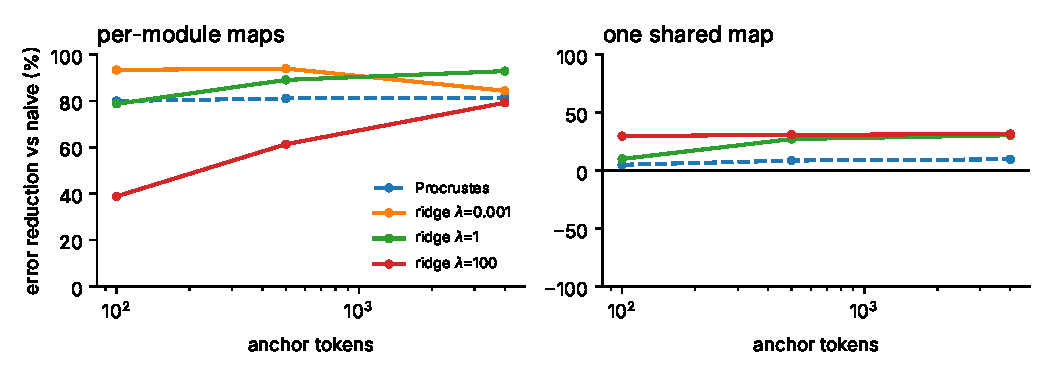
\includegraphics[width=\linewidth]{figures/ablations_synth.pdf}
\caption{Controlled-drift sweep. Error reduction relative to naive transfer as
a function of anchor budget, for ridge at three $\lambda$ and for the
orthogonal solution, with per-module maps (left) and a single shared map
(right). Ridge with light regularization recovers over $90\%$ of the planted
drift from $100$ anchor tokens; the orthogonal solver saturates near $81\%$
regardless of budget; a shared map is at best weakly positive and is harmful at
low $\lambda$.}
\label{fig:ablations_synth}
\end{figure}

\begin{table}[t]
\centering
\small
\begin{tabular}{@{}lrrr@{}}
\toprule
 & \multicolumn{3}{c}{anchor tokens $N$} \\
\cmidrule(l){2-4}
Solver (per-module maps) & 100 & 500 & 4000 \\
\midrule
ridge, $\lambda=10^{-3}$ & 93.4 & \textbf{93.9} & 84.4 \\
ridge, $\lambda=1$       & 78.8 & 89.1 & \textbf{92.9} \\
ridge, $\lambda=100$     & 38.9 & 61.3 & 79.2 \\
orthogonal (Procrustes)  & 80.0 & 81.1 & 81.5 \\
\bottomrule
\end{tabular}
\caption{Error reduction (\%) versus naive transfer on the controlled-drift
problem, per-module maps. Best per column in bold. The single-module
mechanism check (\texttt{validate\_mechanism.py}, $N=4000$, $\lambda=10^{-3}$,
small added noise) reaches $98.6\%$ (ridge) versus $81.4\%$ (orthogonal).}
\label{tab:ablations_synth}
\end{table}

\paragraph{Unconstrained beats orthogonal, and the gap is the non-orthogonal
part of the drift.}
The orthogonal solver plateaus at $80$--$82\%$ error reduction and does not
improve with more anchors: it has found the best rotation, and the residual is
the anisotropic rescaling it cannot represent. Ridge with $\lambda=10^{-3}$
reaches $93$--$94\%$ at $N\le500$, and the single-module mechanism check
reaches $98.6\%$ versus $81.4\%$. The planted drift here is deliberately mild
(singular values within $\pm30\%$ of one). Real version drift has no reason to
be closer to orthogonal, and the real-pair CKA values in \S\ref{sec:drift} are
nonzero precisely because the drift is not a rotation. This is the
quantitative basis for predicting that any method restricted to orthonormal
bases, including subspace projection (\S\ref{sec:method:crosslora}), leaves
part of the recoverable gap on the table. The prediction already holds at the
level of activations on real checkpoints: at the residual stream of
Qwen2-0.5B$\to$Qwen2.5-0.5B, unconstrained maps explain a mean held-out $R^2$
of $0.70$ versus $0.45$ for the best rotation, and win in every layer
(\S\ref{sec:drift:structure}).

\paragraph{Regularization trades fit against sample size in the usual way.}
At $N=100$ anchor tokens for a $64$-dimensional map the regression is barely
over-determined and the lightest regularization wins; at $N=4000$ the
$\lambda=10^{-3}$ solution does worse ($84.4\%$) and $\lambda=1$ is best
($92.9\%$). Heavy regularization ($\lambda=100$) shrinks the map toward zero
and is uniformly worst. The practical rule is to scale $\lambda$ with $N$ or,
equivalently, to select it on held-out anchors, which costs nothing since
anchors are unlabeled and plentiful. We sweep $\lambda$ on the real pair for
the same reason.

\paragraph{Roughly one hundred anchor tokens suffice at this width.}
Per-module ridge reaches $93\%$ from $100$ tokens and gains little beyond
$500$. The number of parameters in a $d\times d$ map grows as $d^2$ while each
anchor token supplies $d$ constraints, so the token budget needed scales
roughly linearly in $d$; for $d=1536$ (the 1.5B pair) this suggests on the
order of a few thousand tokens, which is still a single short forward pass.
%TODO(GPU): confirm with the real anchor-budget sweep.

\paragraph{Drift is module-specific: one shared map does not work.}
Fitting a single $P^{\mathrm{in}},P^{\mathrm{out}}$ on the activations of all
four modules stacked together and applying it everywhere is at best weakly
positive ($31\%$ at $\lambda=100$, $N=4000$) and strongly negative at low
regularization ($-155\%$ to $-351\%$: far worse than naive). The shared
solution averages four unrelated drifts into one map that fits none of them,
and with little regularization it confidently applies the wrong rotation to
every module. The orthogonal shared map is likewise near zero ($5$--$10\%$).
Per-module maps are therefore not an implementation convenience but a
requirement, and the finding carries over to the real pair, where
\S\ref{sec:drift} shows that drift differs by a factor of seven across modules
of the same network.

\subsection{Real pair}
\label{sec:ablations:real}
%TODO(GPU): paper/make_tables.py writes paper/tables/sweeps.tex from the
% results_aligned_ridge_lam*.json / results_crosslora_r*.json sweep files.
% Uncomment the \input once runs/qwen2_to_qwen25_1.5b/ exists.
% \input{tables/sweeps}
On the Qwen2-1.5B\,$\to$\,Qwen2.5-1.5B pair we repeat the solver, $\lambda$,
and anchor-budget sweeps using the cached anchor activations, refitting the
maps and re-evaluating the transplanted adapters without re-extracting
activations, and we additionally sweep the Cross-LoRA truncation rank $k$ so
that the baseline is compared at its best setting rather than only at the
published $k=320$.
